\chapter{إدخال نصّ بشكل أكثر أمانا}

إدخال النصوص في لغة الـ\textenglish{C}
هي من أكثر الأمور حساسية. أنت تعرف الدالة
\InlineCode{scanf}
التي تعرّفنا عليها في الفصول الأولى. ستقول : و أيّ الأدوات ستكون أكثر سهولة و طبيعية منها ؟ لكن جهّز نفسك، بعد هذا الفصل ستقول عنها أي شيء باستثناء "بسيطة".

الذين سيستعملون برنامجك هم بطبيعة الحال بشر. فهناك منهم من يخطئ في كتابة شيء، بينما هناك من يتعمّدون إرباك برنامجك بمعلومات غير منتظرة. فإن طلبت من المستعمل : ما هو عُمرك ؟ من يضمن لك بأنه لن يجيبك بـ:" اسمي فلان و أنا من البلد فلان" ؟

الهدف من هذا الفصل هو تعريفك إلى بعض المشاكل التي يمكن أن نواجهها أثناء استعمالنا للدالة
\InlineCode{scanf}،
و تقديم دالة بديلة أكثر أماناً و هي
\InlineCode{fgets}.

\section{حدود الدالة \texttt{scanf}}

هذه الدالة التي نستعملها جميعاً من الفصول الأولى في الكتاب، هي سلاح ذو حدين :

\begin{itemize}
  \item سهلة الاستعمال حينما نكون في مستوى "مبتدئ" ، و لهذا السبب عرّفتك بها.
  \item لكن الطريقة التي تعمل بها معقّدة و يمكن أن تكون خطيرة في بعض الحالات.
\end{itemize}

ألا يبدو الأمر متناقضا ؟ فإن الدالة
\InlineCode{scanf}
سهلة الاستعمال و في نفس الوقت أكثر تعقيداً مما نتصور، سأريك الحدود التي يمكن لهذه الدالة أن تصل إليها و ذلك بتقديم مثالين واقعيين.

\subsection{إدخال سلسلة محارف تحتوي على فراغات }

لنفرض أننا طلبنا من المستعمل أن يقوم بإدخال سلسلة محارف في الكونسول، و هو يقوم بكتابة فراغ في سلسلته~:

\begin{Csource}
#include <stdio.h>
#include <stdlib.h>
int main(int argc, char *argv[])
{
	char name[20] = {0};
	printf("What's your name ? ");
	scanf("%s", name);
	printf("Ah ! Your name is %s !\n\n", name);
	return 0;
}
\end{Csource}

\begin{Console}
What's your name ? Mathieu Nebra
Ah ! Your name is Mathieu !
\end{Console}

\begin{question}
لماذا اختفت الكلمة
"\textenglish{Nebra}"
؟
\end{question}

ذلك لأن الدالة
\InlineCode{scanf}
تتوقف عن القراءة حينما تصل إلى فراغ، أو رجوع إلى السطر أو محرف جدولة
(\textenglish{tabulation}).
يعني أنك غير قادر على قراءة سلسلة محرفيّة تحتوي على فراغات.

\begin{information}
  في الواقع، الكلمة
  "\textenglish{Nebra}"
  لازالت مخزّنة في الذاكرة، في  شيء نسميه بالمتغير المؤقّت
  (\textenglish{buffer})،
  المرة القادمة عندما نستدعي الدالة
  \InlineCode{scanf}
  فهي ستقوم بقراءة الكلمة
  "\textenglish{Nebra}"
    وحدها الموجودة في المتغير المؤقت.
\end{information}

يمكننا استعمال الدالة
\InlineCode{scanf}
بشكل يسمح لها بقراءة الفراغات، لكن الأمر معقّد جدّا. لمن يصرّ على ذلك، يمكنك إيجاد دروس مفصّلة على الويب، مثل الدرس الأجنبي المتوفّر على هذا الرابط :

\url{http://xrenault.developpez.com/tutoriels/c/scanf/}

\subsection{إدخال سلسلة محارف طويلة للغاية}

يوجد مشكل آخر، أكثر خطورة، و هو
\textbf{تجاوز الذاكرة}.

في الشفرة التي رأيناها، يوجد السطر التالي :

\begin{Csource}
char name[5] = {0};
\end{Csource}

ترى أنني قمت بحجز 5 خانات من أجل الجدول المسمّى
\InlineCode{name}
الذي هو من نوع
\InlineCode{char}.
يعني أننا قادرون على تخزين كلمة من 4 محارف، بينما الحرف الأخير فهو محجوز لعلامة نهاية السلسلة
\InlineCode{\textbackslash 0}.\\
إذا نسيت كلّ هذا فراجع فصل السلاسل المحرفية.

المخطط التالي يمثل المكان الذي هو محجوز للكلمة التي عرّفناها :

\begin{figure}[H]
	\centering
	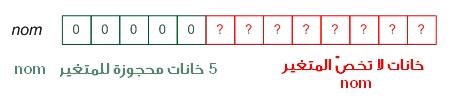
\includegraphics[width=0.5\textwidth]{Chapter_II-10_array}
\end{figure}

ماذا لو كتبنا عددا كبيرا من المحارف بالنسبة للمساحة المتوقّعة لتخزين المتغير ؟

\begin{Console}
What's your name ? Patrice
Ah ! Your name is Patrice !
\end{Console}

ستقول أن كل شيء على ما يرام لكن الواقع أنك بصدد مواجهة أكبر كابوس لدى المبرمجين !

لقد قمنا بـ\emph{تجاوز في الذاكرة}،
 هذا ما نسميه بـ\emph{\textenglish{buffer overflow}}
بالإنجليزية.

كما ترى في المخطط التالي، لقد حجزت 5 خانات لكي تقوم باستعمال 8، ما الذي قامت به الدالة
\InlineCode{scanf}~؟
 لقد قامت بمواصلة الكتابة في الذاكرة وكأن شيئاً لم يحدث ! فلقد استغلّت خانات ليس لها الحق في الكتابة فيها.

\begin{figure}[H]
	\centering
	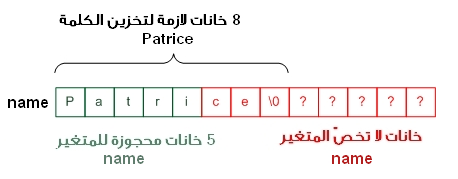
\includegraphics[width=0.5\textwidth]{Chapter_II-10_array_patrice}
\end{figure}

الذي جرى في الحقيقة، هو أن المحارف الزائدة تسببت في مسح معلومات من الذاكرة و استبدالها بهذه المحارف. هذا ما نسميه بالـ\emph{\textenglish{buffer overflow}}.

\begin{figure}[H]
	\centering
	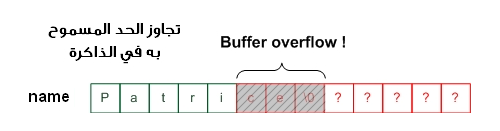
\includegraphics[width=0.5\textwidth]{Chapter_II-10_array_overflow}
\end{figure}

\begin{question}
  لما الأمر خطير ؟
\end{question}

دون الدخول في التفاصيل، لأنه بإمكاننا البدء في محادثة  قدر 50 صفحة و لا نتوقف أبداً، فلنقل بأنه إن لم يقم البرنامج بمعالجة حالات كهذه، فالمستعمل سيقوم بكتابة ما يحلو له و تخريب المعلومات المتواجدة في الخانات التالية من الذاكرة. أي أنه قادر على كتابة شفرة في تلك الخانات و برنامجك سيقوم بتشغيل تلك الشفرات و كأنها تابعة له، و هذا ما نسميه بالهجوم عبر المتغير المؤقت
(\textenglish{Buffer overflow attack})،
نوع من الهجومات المعروفة عند القراصنة، و لكنه صعب التحقيق.\\
إذا كنت مهتماً بهذا الموضوع، يمكنك قراءة المقال التالي من ويكيبيديا (حذار، إنّه مع ذلك معقد جدا) :

\url{http://fr.wikipedia.org/wiki/D%C3%A9passement_de_tampon}

الهدف من هذا الفصل هو تأمين قراءة البيانات و ذلك بمنع المستعمل من تجاوز الذاكرة و إحداث
\textenglish{buffer overflow}.
بالطبع كان بإمكاننا تعريف جدول كبير للغاية (10,000 خانة) لكن هذا لا يحلّ المشكل فالشخص الذي يريد الوصول إلى الذاكرة ما عليه سوى إدخال سلسلة يتجاوز طولها 10,000 محرف و سيعمل هجومه كما يريد.

الشيء المحزن هو أن معظم المبرمجين لا ينتبهون دائما لهذه الأخطاء، و لو أنهم قاموا بكتابة الشفرة من المرة الأولى بشكل نظيف و صحيح، لما ظهرت كثير من الثغرات التي نتحدّث عنها اليوم.

\section{استرجاع سلسلة محارف}

توجد العديد من الدوال القياسيّة في لغة
\textenglish{C}
التي تسمح باسترجاع سلسلة نصّيّة. إضافة إلى الدالة
\InlineCode{scanf}،
و التي من الصعب دراستها هنا، لدينا :

\begin{itemize}
  \item \InlineCode{gets}:
دالة تقرأ سلسلة محرفيّة كاملة لكنها خطيرة جدّا لأنها لا تعالج مشكل الـ\textenglish{buffer overflow}.
  \item \InlineCode{fgets} :
 تشبه الدالة
\InlineCode{gets}
لكنها تحمي البرنامج و ذلك بالتحكم في عدد المحارف المكتوبة في الذاكرة.
\end{itemize}

أعتقد أن الأمر مفهوم : على الرغم من أنها دالّة قياسيّة في الـ\textenglish{C}،
\InlineCode{gets}
هي دالّة خطيرة  جدّا. كل البرامج الّتي تستخدمها عرضة لأن يكونوا ضحايا الـ\textenglish{buffer overflow}.

سنرى كيف تعمل الدالة
\InlineCode{fgets}،
و كيف نستعملها في برامجنا الخاصّة في مكان الدالة
\InlineCode{scanf}.

\subsection{الدالّة \texttt{fgets}}

نموذج هذه الدالة، المتواجد في المكتبة
\InlineCode{stdio.h}
هو :

\begin{Csource}
char *fgets(char *str, int num, FILE *stream);
\end{Csource}

من المهم أن نفهم هذا النموذج. معاملات الدالة هي التالية :

\begin{itemize}
  \item \InlineCode{str} :
مؤشّر نحو جدول في الذاكرة، أين ستتمكن الدالة من كتابة النص المدخل من طرف المستخدم.
  \item \InlineCode{num} :
حجم الجدول
\InlineCode{str}
المرسل كمعامل أوّل.

لاحظ أنه لو قمت بحجز جدول من
\InlineCode{char}،
فإن الدالة
\InlineCode{fgets}
ستقرأ 9 محارف على الأكثر (آخر خانة محجوزة للمحرف
\InlineCode{\textbackslash 0}
المشير إلى نهاية السلسلة).
  \item \InlineCode{stream} :
مؤشّر نحو الملف الذي سنقرأ منه. في حالتنا "الملف المراد قراءته" هو الإدخال القياسي
(\textenglish{Standard input})،
أي لوحة المفاتيح. لطلب قراءة الإدخال القياسي نرسل المؤشّر
\InlineCode{stdin}
المعرّف تلقائيّا في الملفات الرأسيّة للمكتبة القياسيّة للـ\textenglish{C}
ليشير إلى لوحة المفاتيح. مع ذلك، يمكن استخدام
\InlineCode{fgets}
لقراءة الملفّات، كما رأينا في الفصل الخاص بالملفّات.
\end{itemize}

الدالة ستقوم بإرجاع نفس المؤشّر
\InlineCode{str}
للإشارة إلى إن كانت القراءة قد تمت بشكل صحيح أم لا. يكفي إذا أن نختبر ما إن كانت قيمة هذا المؤشّر تساوي
\InlineCode{NULL}،
فإن كانت كذلك، فهناك خطأ.

فلنجرّب !

\begin{Csource}
#include <stdio.h>
#include <stdlib.h>
int main(int argc, char *argv[])
{
	char name[10];
	printf("What's your name ? ");
	fgets(name, 10, stdin);
	printf("Ah ! Your name is %s !\n\n", name);
	return 0;
}
\end{Csource}

\begin{Console}
What's your name ? NEBRA
Ah ! Your name is NEBRA
!
\end{Console}

الدالة تعمل بشكل جيد، مع تفصيل بسيط : عندما تضغط على زر الإدخال، تقوم
\InlineCode{fgets}
بالاحتفاظ بـ\InlineCode{\textbackslash n}
الموافق، هذا ما يفسّر الرجوع إلى السطر بعد الكلمة
"\textenglish{NEBRA}"
كما يظهر في الكونسول.

لا يمكننا أن نمنع هذه الدالة من كتابة المحرف
\InlineCode{\textbackslash n}
لأن الدالة تعمل هكذا. بالمقابل، هذا لا يمنع كتابتنا لدالة خاصّة بالإدخال تقوم نفسها باستدعاء
\InlineCode{fgets}
و حذف ذلك المحرف !

\subsection{كتابة دالتك الخاصّة بالإدخال باستخدام \texttt{fgets}}

ليس صعباً جدّا أن نقوم بكتابة دالة خاصة بك تقوم ببعض التصحيحات من أجلك في كلّ مرّة.

سنسمّي هذه الدالّة
\InlineCode{read}.
ستقوم بإرجاع القيمة 0 إن كان هناك خطأ و 1 إن لم يكن.

\subsubsection{حذف الرجوع إلى السطر \texttt{\textbackslash n}}

الدالة
\InlineCode{read}
تستدعي
\InlineCode{fgets}،
إذا تمّ كلّ شيء على ما يرام، ستبحث عن المحرف
\InlineCode{\textbackslash n}
بمساعدة الدالة
\InlineCode{strchr}
الّتي يفترض بك معرفتها. إذا تمّ العثور على
\InlineCode{\textbackslash n}،
فستستبدله بـ\InlineCode{\textbackslash 0}
(نهاية السلسلة) لتجنّب الاحتفاظ بـ"علامة الإدخال".

هاهي الشفرة علّقت عليها خطوة بخطوة :

\begin{Csource}
#include <stdio.h>
#include <stdlib.h>
#include <string.h> // Think to include string.h for strchr()
int read(char *string, int length)
{
	char *enterPosition = NULL;
	// We read the text
	if (fgets(string, length, stdin) != NULL)  // No error ?
	{
    		enterPosition = strchr(string, '\n'); // We search for the "Enter"
    		if (enterPosition != NULL) // If we find the \n
    		{
        			*enterPosition = '\0'; // We replace the character by \0
    		}
    		return 1; // We return 1 if there's no error
	}
	else
	 {
    		return 0; // We return 0 if there's error
	 }
}
\end{Csource}

ستلاحظ أنه بالإمكان استدعاء الدالة
\InlineCode{fgets}
مباشرة داخل
\InlineCode{if}.
هذا اختصار كتابي، كي لا أستعمل مؤشّرا يستقبل القيمة المُرجعة من الدالة ثم أختبر قيمته إن كانت
\InlineCode{NULL}
أم لا.

انطلاقا من
\InlineCode{if}
الأول، أعرف هل
\InlineCode{fgets}
عملت على ما يرام أم حدث مشكل ما (قام المستخدم بادخال محارف أكبر من العدد المسموح به).

إذا تم كل شيء بشكل جيد، سأذهب للبحث عن الـ\InlineCode{\textbackslash n}
باستعمال الدالة
\InlineCode{strchr}
ثم استبداله بالمحرف
\InlineCode{\textbackslash 0}
كما في الشكل التالي.

\begin{figure}[H]
	\centering
	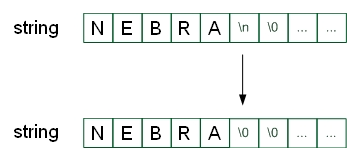
\includegraphics[width=0.3\textwidth]{Chapter_II-10_string}
\end{figure}

هذا المخطط يبيّن أن السلسلة الّتي تمت قراءتها من طرف الدالة
\InlineCode{fgets}
هي
"\InlineCode{NEBRA\textbackslash n\textbackslash 0}"،
ثم قمنا باستبدال الـ\InlineCode{\textbackslash n}
بـ\InlineCode{\textbackslash 0}
و هذا ما أعطانا
"\InlineCode{NEBRA\textbackslash 0\textbackslash 0}".\\
ليس مشكلا أن توجد علامتا
\InlineCode{\textbackslash 0}
متتابعتين. الحاسوب سيتوقف عند الإشارة الأولى و يعتبرها نهاية السلسلة.

و النتيجة ؟ حسنا، لقد عملت بشكل جيّد.

\begin{Csource}
  int main(int argc, char *argv[])
  {
  	char name[10];
  	printf("What's your name ? ");
  	read(name, 10);
  	printf("Ah ! Your name is %s !\n\n", name);
  	return 0;
  }
\end{Csource}

\begin{Console}
What's your name ? NEBRA
Ah ! Your name is NEBRA !
\end{Console}

\subsubsection{تفريغ المتغيّر المؤقّت}

لم نصل بعد إلى نهاية الأمور المزعجة.\\
نحن لم نقم بتحليل الحالة التي يقوم فيها المستعمل بإدخال محارف أكثر من ما هو مسموح به !

\begin{Console}
What's your name ? Jean Edouard Albert 1er
Ah ! Your name is Jean Edou !
\end{Console}

بما أن الدالة
\InlineCode{fgets}
تدعم الحماية، فهي توقفت عند الحرف التاسع الذي قام المستعمل بإدخاله لأنّنا حجزنا جدولا من 10 محارف (يجب عدم نسيان أنّ العاشر محجوز لإشارة نهاية السلسلة).
المشكل هو أن بقيّة السلسلة الّتي لم تتم قراءتها.
"\textenglish{ard Albert 1er}"
لم تختف ! و إنّما لازالت موجودة في المتغير المؤقّت. هذا المتغير المؤقت هو مكان في الذاكرة يعمل كوسيط بين لوحة المفاتيح و الجدول الّذي سيتم تخزين السلسلة فيه. في الـ\textenglish{C}،
لدينا مؤشّر نحو المتغير المؤقت، و هو
\InlineCode{stdin}
الذي تكلمنا عنه قبل قليل.

أعتقد أن مخططا صغيرا سيساعد على توضيح الأمور.

\begin{figure}[H]
	\centering
	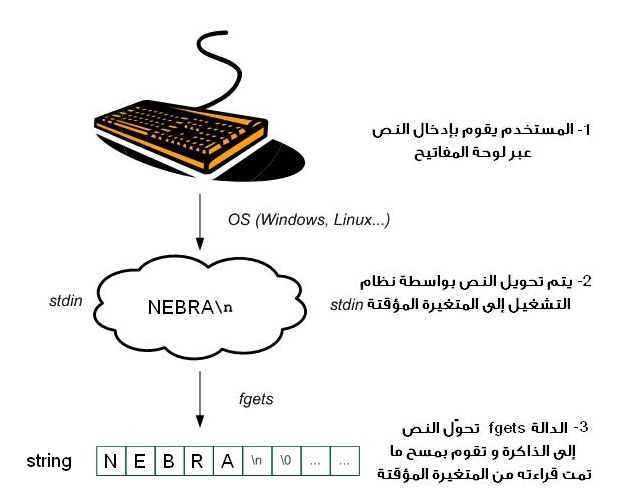
\includegraphics[width=0.6\textwidth]{Chapter_II-10_buffer}
\end{figure}

حينما يقوم المستعمل بإدخال نص بلوحة المفاتيح، فإن نظام التشغيل 
(\textenglish{Windows}
مثلا) يقوم بنسخ النص مباشرة في المتغير المؤقّت
\InlineCode{stdin}.

مهمة الدالة
\InlineCode{fgets}
هي إحضار المحارف الموجودة في المتغير المؤقت ووضعها في الذاكرة التي قمت أنت بتحديدها (الجدول
\InlineCode{string}).\\
بعد القيام بعملها، تمسح ما قامت بنسخه من المتغير المؤقّت.

إذا عمل كل شيء على ما يرام، فالدالة
\InlineCode{fgets}
ستقوم بإفراغ كل محتوى المتغير المؤقّت، أي أن هذا الأخير سيكون فارغاً بعد استدعاء الدالة. لكن في الحالة التي يقوم المستخدم بإدخال كثير من المحارف لا يمكن أن يسعها المكان المحجوز لها، فإنه يتم مسح الحروف التي تمت قراءتها فقط، و بالتالي بعد استدعاء الدالة
\InlineCode{fgets}
فإن المتغير المؤقّت يحتوي دائما المحارف المتبقّية !

فلنجرّب مع سلسلة كبيرة :

\begin{Csource}
  int main(int argc, char *argv[])
  {
  	char name[10];
  	printf("What's your name ? ");
  	read(name, 10);
  	printf("Ah ! Your name is %s !\n\n", name);
  	return 0;
  }
\end{Csource}

\begin{Console}
  What's your name ? Jean Edouard Albert 1er
  Ah ! Your name is Jean Edou !
\end{Console}

الدالة
\InlineCode{fgets}
قامت بنسخ المحارف التسعة الأولى كما كان متوقّعا. المشكل هو أن المحارف المتبقية لازالت في المتغير المؤقت !

\begin{figure}[H]
	\centering
	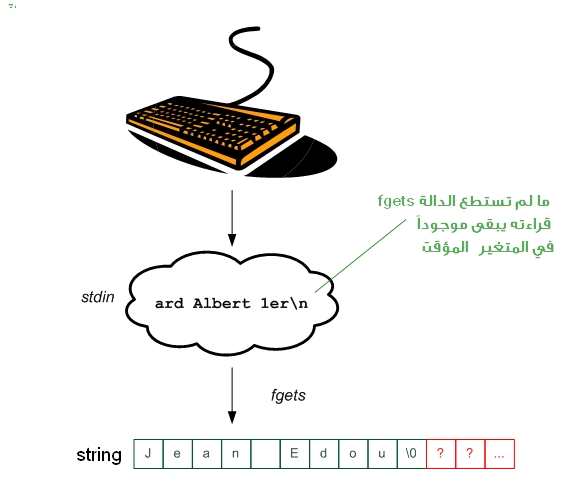
\includegraphics[width=0.6\textwidth]{Chapter_II-10_buffer_rest}
\end{figure}

هذا يعني أنه لو استدعينا الدالة
\InlineCode{fgets}
مرة أخرى فإنها ستقوم بقراءة ما كان متبقّيا في المتغير المؤقت !

فلنجرّب هذه الشفرة :

\begin{Csource}
int main(int argc, char *argv[])
{
 	char name[10];
 	printf("What's your name ? ");
 	read(name, 10);
 	printf("Ah ! Your name is %s !\n\n", name);
 	read(name, 10);
 	printf("Ah ! Your name is %s !\n\n", name);
 	return 0;
}
\end{Csource}

نحن نقوم باستدعاء الدالة
\InlineCode{read}
مرّتين لكنك ستلاحظ أنّه لن يتم السماح لك بإدخال اسمك مرتين، وذلك لأن الدالة
\InlineCode{fgets}
لن تطلب من المستخدم إدخال أيّ نصّ في المرّة الثانية لأنّها ستجده في المتغير المؤقت !

\begin{Console}
  What's your name ? Jean Edouard Albert 1er
  Ah ! Your name is Jean Edou !
  Ah ! Your name is ard Alber !
\end{Console}

إذا قام المستعمل بإدخال محارف كثيرة، فإن الدالة
\InlineCode{fgets}
ستحمي البرنامج من مشكل تجاوز الذاكرة، لكن يبقى دائما آثار النصّ في المتغير المؤقت. لذا يجب تفريغ هذا الأخير.

سنقوم إذا بتحسين عمل الدالة
\InlineCode{read}،
و سنقوم في الحالات التي تتطلب ذلك باستدعاء دالة نسميها
\InlineCode{clearBuffer}،
لكي نتأكد من تفريغ المتغير المؤقت في حال ما احتوى على محارف زائدة :

\begin{Csource}
void clearBuffer()
{
 	int c = 0;
 	while (c != '\n' && c != EOF)
 	{
     		c = getchar();
 	}
}
int read(char *string, int length)
{
 	char *enterPosition = NULL;
 	if (fgets(string, length, stdin) != NULL)
 	{
     		enterPosition = strchr(string, '\n');
     		if (enterPosition != NULL)
     		{
         			*enterPosition = '\0';
     		}
     		else
     		{
         			clearBuffer();
     		}
     		return 1;
 	}
 	else
 	{
     		clearBuffer();
     		return 0;
	}
}
\end{Csource}

الدالة
\InlineCode{read}
تستدعي الدالة
\InlineCode{clearBuffer}
في حالتين :

\begin{itemize}
  \item السلسلة المدخلة طويلة جداً (يمكننا أن نعرف ذلك بعدم وجود الإشارة
\InlineCode{\textbackslash 0}
في السلسلة المنسوخة).
  \item إذا حدث أي خطأ مهما كان، يجب تفريغ محتوى المتغير المؤقت لأسباب حماية لكي لا يبقى شيء هناك.
\end{itemize}

الدالة
\InlineCode{clearBuffer}
قصيرة لكنها عميقة. فهي تقرأ المتغير المؤقت محرفاً محرفاً باستعمال الدالة
\InlineCode{getchar}.
هذه الدالة تقوم بإرجاع
\InlineCode{int}
(و ليس
\InlineCode{char}،
سوف تعرف السبب لاحقا، أيّا يكن).\\
سنكتفي نحن باسترجاع القيمة في متغير
\InlineCode{c}
من نوع
\InlineCode{int}.
نقوم بحلقة تكرارية مادمنا لم نقرأ بعد المحرف
\InlineCode{\textbackslash 0}
 أو الرمز
\InlineCode{EOF}
(نهاية الملف) و هما يعنيان : لقد وصلت إلى نهاية المتغير المؤقت. سنتوقّف عند الوصول إلى أحد هذين المحرفين.

يبدو عمل الدالة
\InlineCode{clearBuffer}
صعباً قليلاً لكنها تقوم بعملها. لا تتردد في تكرار قراءة الشرح عدة مرات من أجل الفهم الجيد.

\section{تحويل سلسلة محرفيّة إلى عدد}

دالتنا
\InlineCode{read}
هي فعالة و قويّة الآن، لكنها تجيد قراءة النصوص فقط. ستتساءل حتما : "لكن كيف نقوم باسترجاع عدد ؟"

الحقيقة أن الدالة
\InlineCode{fgets}
هي دالة مبدئية. مع
\InlineCode{fgets}
لا يمكن قراءة سوى النصوص، و لكن توجد دوال أخرى تقوم بتحويل النص إلى عدد.

\subsection{\texttt{strtol} : تحويل سلسلة محرفيّة إلى \texttt{long}}

نموذج هذه الدالة خاص نوعاً ما :

\begin{Csource}
long strtol(const char *start, char **end, int base);
\end{Csource}

الدالة ستقوم بقراءة السلسلة المحرفيّة المرسلة إليها
(\InlineCode{start})
و ستحاول تحويلها إلى
\InlineCode{long}
باستعمال الأساس
(\InlineCode{base})
المحدد (غالباً ما نستعمل الأساس 10، لأننا نستعمل الأرقام من 0 إلى 9، و لهذا ضع مكانه العدد 10). ستقوم بإرجاع العدد الذي نجحت في قراءته.\\
بالنسبة لمؤشر المؤشر
\InlineCode{end}،
فالدالة ستقوم باستغلاله لإرجاع أول محرف صادفته و لم يكن رقماً. لكننا لسنا بحاجة إليه، فلنكتفي بوضع
\InlineCode{NULL}
مكانه لنقول أننا لا نريد استرجاعه.

على السلسلة المحرفيّة أن تبدأ برقم، فبعد الأرقام كل شيء يتم تجاهله. يمكن أن تكون مسبوقة بفراغات.\\
هذه أمثلة للفهم الجيد :

\begin{Csource}
long i;
i = strtol("148", NULL, 10); // i = 148
i = strtol("148.215", NULL, 10); // i = 148
i = strtol(" 148.215", NULL, 10); // i = 148
i = strtol(" 148+34", NULL, 10); // i = 148
i = strtol(" 148 dead leaves", NULL, 10); // i = 148
i = strtol( " There are 148 dead leaves", NULL, 10 ); // i = 0 (error : The string doesn't start with a number)
\end{Csource}

كل السلاسل التي تبدأ برقم (أو ربما بفراغات قبله) سيتم تحويلها إلى
\InlineCode{long}
حتى الوصول إلى محرف غير مقبول (نقطة، فاصلة، علامة استفهام، زائد، إلخ).

بالنسبة لسلسلة لا تبدأ بأرقام و أو بفراغات تليها أرقام، فلا يمكن تحويلها و بالتالي تقوم الدالة بإرجاع القيمة~0.

يمكننا كتابة الدالة
\InlineCode{readLong}،
و التي تقوم باستدعاء الدالة
\InlineCode{read}
(لقراءة النص)، و بعد ذلك تحويل النص إلى عدد :

\begin{Csource}
long readLong()
{
 	char textNumber[100] = {0}; // 100 cells are sufficient
 	if (read(textNumber, 100))
 	{
     		// If we read the text without problems, we convert textNumber to long and we return it
    		 return strtol(textNumber, NULL, 10);
 	}
 	else
 	{
    		 // If there's a problem, we return 0
     		return 0;
	 }
}
\end{Csource}

يمكنك تجريب الشفرة داخل
\InlineCode{main}
بسيط.

\begin{Csource}
int main(int argc, char *argv[])
{
 	long age = 0;
 	printf("How old are you ? ");
 	age = readLong();
 	printf("Ah ! You are %d years old !\n\n", age);
 	return 0;
}
\end{Csource}

\begin{Console}
How old are you ? 18
Ah ! You are 18 years old!
\end{Console}

\subsection{\texttt{strtod} تحويل سلسلة محرفيّة إلى \texttt{double}}

الدالة
\InlineCode{strtod}
مطابقة للدالة
\InlineCode{strtol}،
الفرق الوحيد هو أنها ستحاول قراءة عدد عشريّ و إرجاع
\InlineCode{double}.

\begin{Csource}
double strtod(const char *start, char **end);
\end{Csource}

تجد أن المعامل الثالث
\InlineCode{base}
اختفى هنا، بينما يبقى مؤشّر المؤشّر
\InlineCode{end}
الّذي لا يفيدنا في شيء.

على خلاف الدالة السابقة، فإن هذه الدالة ستأخذ في الحسبان "النقطة" العشرية. عندما أقول نقطة يعني أن الدالة لا تقبل الفاصلة
"\textenglish{,}"
(يبدو أنّها مبرمجة من طرف ناطقين بالإنجليزية).

فلتقم بكتابة الدالة
\InlineCode{readDouble}
بنفسك. إن كتابتها مماثلة للدالة
\InlineCode{readLong}،
الاختلاف الوحيد هو أنها ستستدعي الدالة
\InlineCode{strtod}
ثم ستقوم بإرجاع قيمة
\InlineCode{double}.

يعني أنك ستكتب التالي في الكونسول :

\begin{Console}
  What's your weight ? 67.4
  Ah ! Your weight is 67.400000 kg !
\end{Console}


حاول بعد ذلك تعديل الدالة
\InlineCode{readDouble}
لتقبل الفاصلة أيضاً كفاصل عشري. إن الأمر بسيط : فقط قم باستبدال كل تكرار للمحرف
"\InlineCode{,}"
بالمحرف
"\InlineCode{.}"
(بالاستعانة بالدالة
\InlineCode{strchr})،
ثم قم ببعث النص الجديد إلى الدالة
\InlineCode{strtod}.

\section*{ملخّص}

\begin{itemize}
  \item الدالة
\InlineCode{scanf}
بالرغم من أنها تبدو سهلة و طبيعية إلا أنها معقّدة و تفرض علينا بعض الحدود. فمثلاً، هي لا تقبل قراءة نص يحتوي فراغات.
  \item نقول أننا تسببنا في الـ\textenglish{buffer overflow}
إذا تجاوزنا المساحة المخصصة في الذاكرة، فمثلاً لو قام المستخدم بإدخال 10 محارف و نحن قد حجزنا 5 خانات فقط.
  \item الحل الأمثل هو استدعاء الدالة
\InlineCode{fgets}
لتقوم باسترجاع النص الذي يُدخله المستعمل.
  \item يجب أن تتجنب استعمال الدالة
\InlineCode{gets}
بأي ثمن لأنّها لا تحمي من الـ\textenglish{buffer overflow}.
  \item يمكنك كتابة دالة خاصة بك، تقوم باستدعاء الدالة
\InlineCode{fgets}
كما فعلنا لكيّ تحسّن عملها.
\end{itemize}
